\documentclass[aspectratio=169,10pt]{beamer}

\usepackage[T1]{fontenc}
\usepackage{lmodern}
\usepackage{amsmath}
\usepackage{booktabs}
\usepackage{graphicx}
\usepackage[percent]{overpic}
\usepackage{xcolor}

\definecolor{CDetBlue}{HTML}{17365D}
\definecolor{CDetLightBlue}{HTML}{DCEAF7}
\definecolor{CDetOrange}{HTML}{D97706}
\definecolor{CDetGray}{HTML}{4B5563}
\definecolor{CDetGreen}{HTML}{287A52}

\usetheme{default}
\usefonttheme{professionalfonts}
\setbeamercolor{normal text}{fg=black,bg=white}
\setbeamercolor{structure}{fg=CDetBlue}
\setbeamercolor{frametitle}{fg=white,bg=CDetBlue}
\setbeamercolor{title}{fg=white}
\setbeamercolor{subtitle}{fg=CDetLightBlue}
\setbeamercolor{alerted text}{fg=CDetOrange}
\setbeamercolor{block title}{fg=white,bg=CDetBlue}
\setbeamercolor{block body}{fg=black,bg=CDetLightBlue!45}
\setbeamertemplate{navigation symbols}{}
\setbeamertemplate{itemize item}{\color{CDetOrange}$\blacktriangleright$}
\setbeamertemplate{itemize subitem}{\color{CDetBlue}$\bullet$}
\setbeamertemplate{frametitle}{%
  \nointerlineskip
  \begin{beamercolorbox}[wd=\paperwidth,ht=0.78cm,dp=0.22cm,leftskip=0.48cm]{frametitle}
    \usebeamerfont{frametitle}\insertframetitle
  \end{beamercolorbox}}
\setbeamertemplate{footline}{%
  \leavevmode
  \hbox{%
    \begin{beamercolorbox}[wd=.82\paperwidth,ht=0.28cm,dp=0.14cm,leftskip=0.45cm]{author in head/foot}%
      \color{CDetGray}\scriptsize CDet for GEp-V \hspace{0.7em} APS DNP 2026
    \end{beamercolorbox}%
    \begin{beamercolorbox}[wd=.18\paperwidth,ht=0.28cm,dp=0.14cm,rightskip=0.45cm plus1fil]{date in head/foot}%
      \color{CDetGray}\scriptsize\hfill\insertframenumber/\inserttotalframenumber
    \end{beamercolorbox}}}
\setbeamersize{text margin left=0.55cm,text margin right=0.55cm}

\newcommand{\result}[1]{\textcolor{CDetGreen}{\textbf{#1}}}
\newcommand{\lesson}[1]{\textcolor{CDetOrange}{\textbf{#1}}}
\newcommand{\assetroot}{../../../../..}

\title{The Coordinate Detector in GEp-V}
\subtitle{}
\author[Benjamin Spaude et al.]{Benjamin Spaude (presenter)\\[0.12cm]
Todd Averett, Edward Brash, Peter Monaghan, Ralph Marinaro}
\institute{SBS Collaboration}
\date{APS Division of Nuclear Physics Meeting, 2026}

\begin{document}

% Suggested pace: 0:25
\begin{frame}[plain]
  \begin{beamercolorbox}[wd=\paperwidth,ht=\paperheight,sep=0pt]{frametitle}
    \color{white}
    \vspace{1.35cm}\hspace{0.75cm}
    \begin{minipage}{0.86\paperwidth}
      {\LARGE\bfseries\inserttitle\par}
      \vspace{0.35cm}
      {\large\color{CDetLightBlue}\insertsubtitle\par}
      \vfill
      {\normalsize\insertauthor\par}
      {\small\color{CDetLightBlue}\insertinstitute\par}
      {\small\color{CDetLightBlue}\insertdate\par}
      \vspace{1.25cm}
    \end{minipage}
  \end{beamercolorbox}
\end{frame}

% Suggested pace: 0:55
\begin{frame}{GEp-V: the proton form-factor ratio at high $Q^2$}
\begin{columns}[T,onlytextwidth]
  \column{0.55\textwidth}
  \begin{itemize}
    \item GEp-V measures the proton elastic form-factor ratio $G_E^p/G_M^p$ through recoil polarization.
    \item The high-$Q^2$ regime provides a sensitive test of QCD-inspired models of proton structure.
    \item The useful elastic signal is rare, and must be distinguished from both inelastic and electromagnetic background seen in the open-geometry apparatus.
  \end{itemize}
  \vspace{0.25cm}
  \begin{block}{Experimental requirement}
    Identify an electron and proton that satisfy the two-arm elastic kinematics, then measure the proton polarization.
  \end{block}
  \column{0.41\textwidth}
  \vspace{0.68cm}
  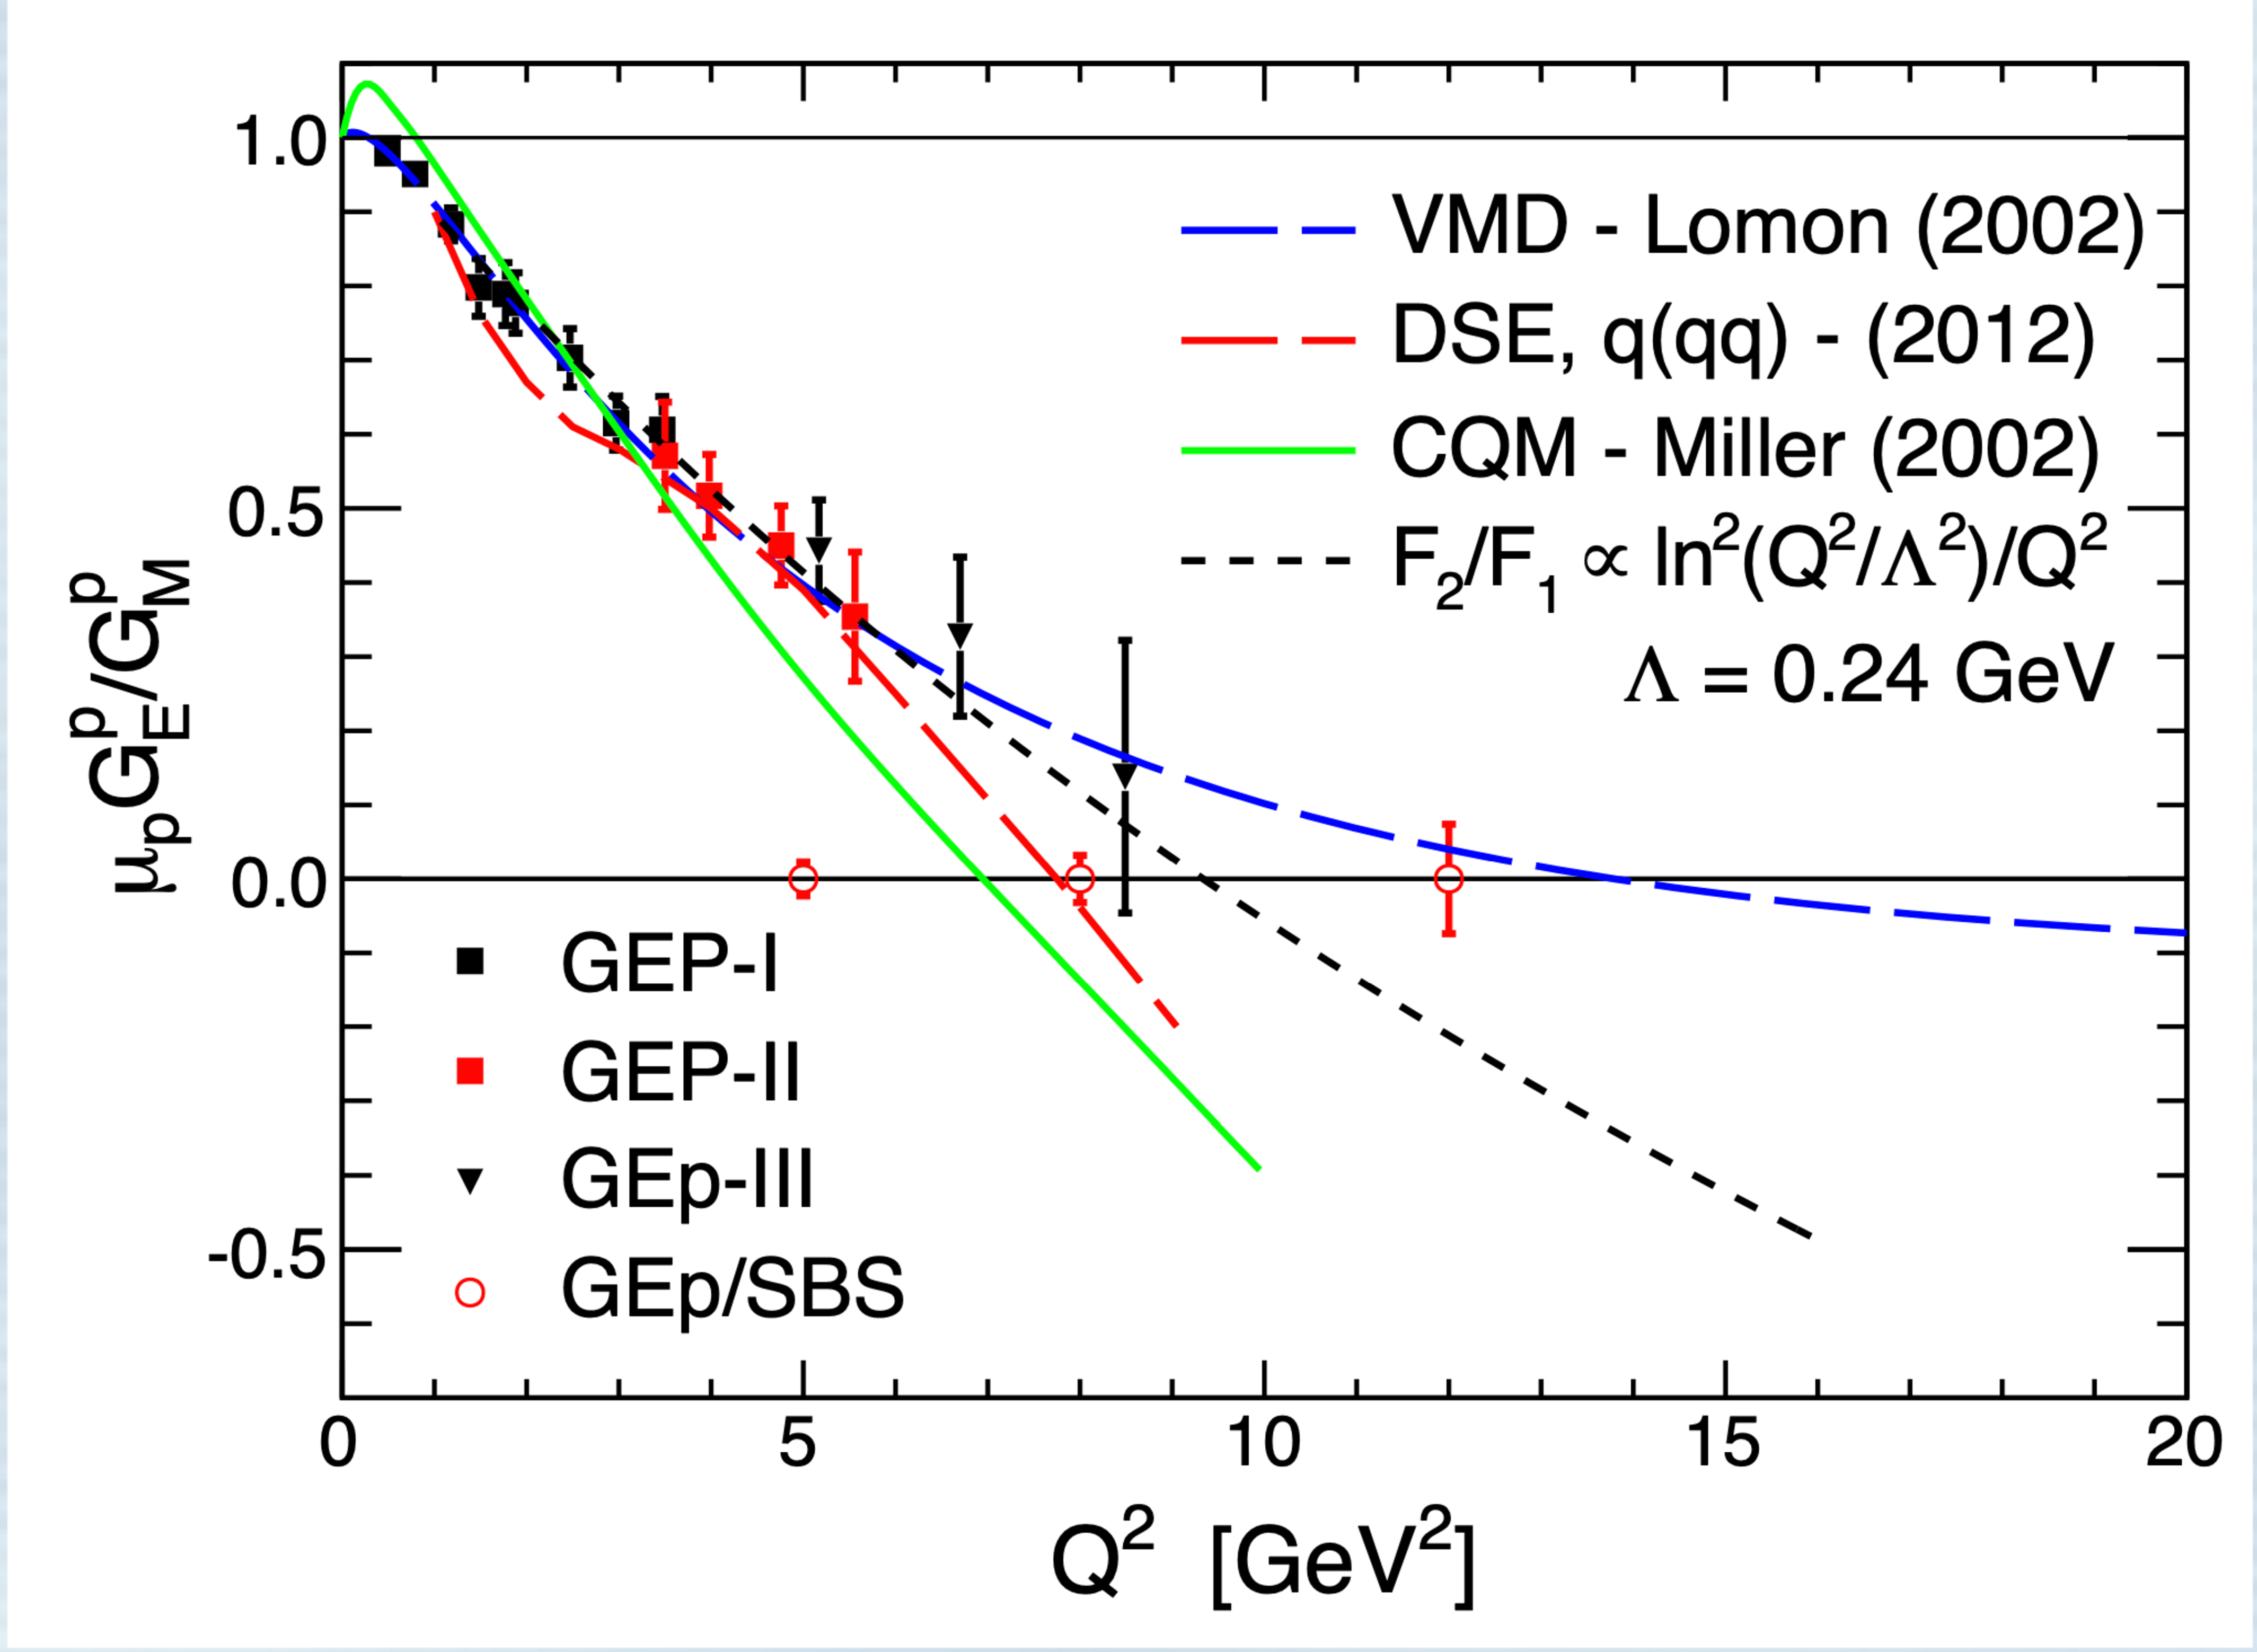
\includegraphics[width=\linewidth,height=0.73\textheight,keepaspectratio]{assets/GEp_GMp_results.pdf}
\end{columns}
\end{frame}

% Suggested pace: 1:05
\begin{frame}{GEp-V experimental layout}
\begin{columns}[T,onlytextwidth]
  \column{0.54\textwidth}
  \centering
  \vspace{0.48cm}
  \begin{overpic}[width=0.94\linewidth]{assets/GEpV_full_layout_clean.png}
    \put(38,73){\colorbox{white}{\textcolor{CDetBlue}{\bfseries\small Electron arm}}}
    \put(53,8){\colorbox{white}{\textcolor{CDetBlue}{\bfseries\small Proton Arm}}}
  \end{overpic}

  \column{0.42\textwidth}
  \footnotesize
  \textbf{Elastic-event selection}
  \begin{itemize}
    \item ECal measures the scattered-electron energy and position.
    \item Two CDet layers add a short tracking lever arm.
    \item The combined trajectory constrains the electron out-of-plane angle and the target association.
  \end{itemize}
  \vspace{0.03cm}
  \textbf{Front-tracker region of interest}
  \begin{itemize}
    \item Electron-arm information predicts where the recoil proton should appear.
    \item A smaller GEM search region can reject unrelated hits.
    \item Reducing the combinatorics may also shorten reconstruction in the high-occupancy, open geometry.
  \end{itemize}
\end{columns}
\vspace{0.10cm}
\centering
\small\lesson{CDet links electron identification to the proton-arm tracking problem.}
\end{frame}

% Suggested pace: 0:55
\begin{frame}{CDet: two layers of segmented scintillator}
\begin{columns}[T,onlytextwidth]
  \column{0.62\textwidth}
  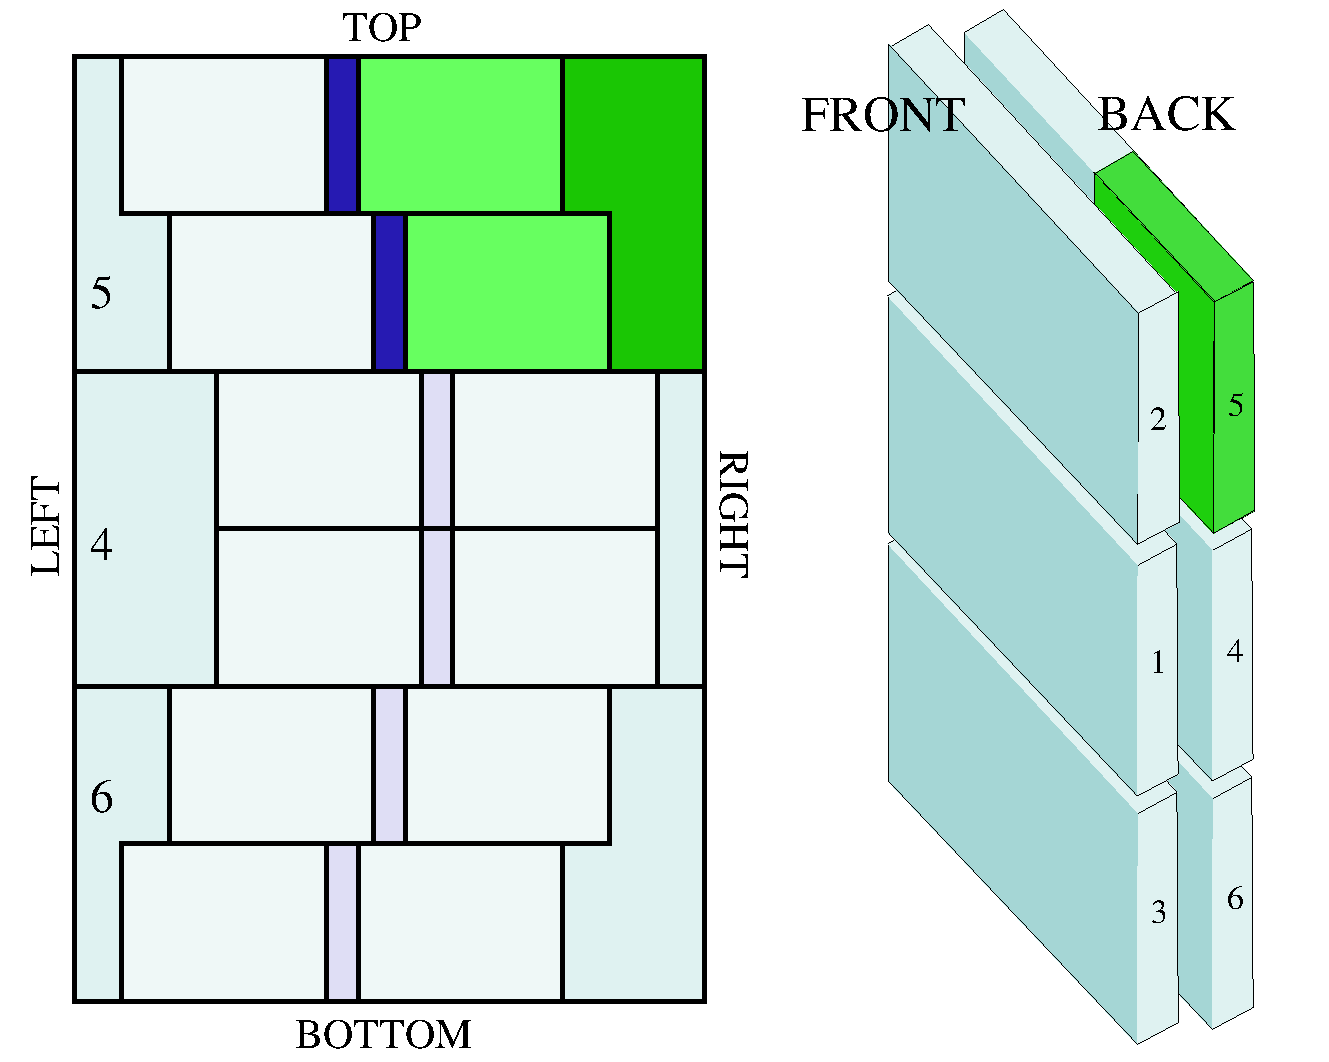
\includegraphics[width=\linewidth,height=0.73\textheight,keepaspectratio]{assets/CDet_full_detector_schematic.png}
  \column{0.34\textwidth}
  \begin{itemize}
    \item 168 scintillator bars in two layers
    \item 84 half-bars per layer
    \item Wavelength-shifting fibers carry light to multi-anode PMTs
    \item 16 pixels per half-bar give 2,688 logical channels
  \end{itemize}
  \vspace{0.2cm}
  \begin{block}{Measured quantities}
    Leading-edge time and trailing-edge time for each discriminator pulse.
  \end{block}
\end{columns}
\end{frame}

% Suggested pace: 1:10
\begin{frame}{The central challenge: hundreds of background hits}
\begin{columns}[T,onlytextwidth]
  \column{0.56\textwidth}
  \begin{itemize}
    \item Lower-energy electrons and photons reach CDet despite the aluminum shielding in front of the detector.
    \item At $I=20~\mu\mathrm{A}$ on a 15 cm liquid-hydrogen target, simulations and initial analysis indicate approximately
      \begin{itemize}
        \item \textbf{500 hits/event} in Layer 1,
        \item \textbf{250 hits/event} in Layer 2,
      \end{itemize}
      within a 60 ns readout window around the coincidence-trigger timing signal.
    \item These occupancies remain after the hardware thresholds are applied.
  \end{itemize}
  \column{0.40\textwidth}
  \begin{block}{NINO threshold}
    The threshold corresponds to roughly 50\% of the energy deposited by a minimum-ionizing, high-energy electron.
  \end{block}
  \vspace{0.22cm}
  \begin{block}{Analysis consequence}
    Timing alone cannot distinguish every signal hit from the large accidental population. Geometry and cross-detector consistency are essential.
  \end{block}
\end{columns}
\end{frame}

% Suggested pace: 1:00
\begin{frame}{TDC-only readout: time over threshold carries the charge information}
\begin{columns}[T,onlytextwidth]
  \column{0.56\textwidth}
  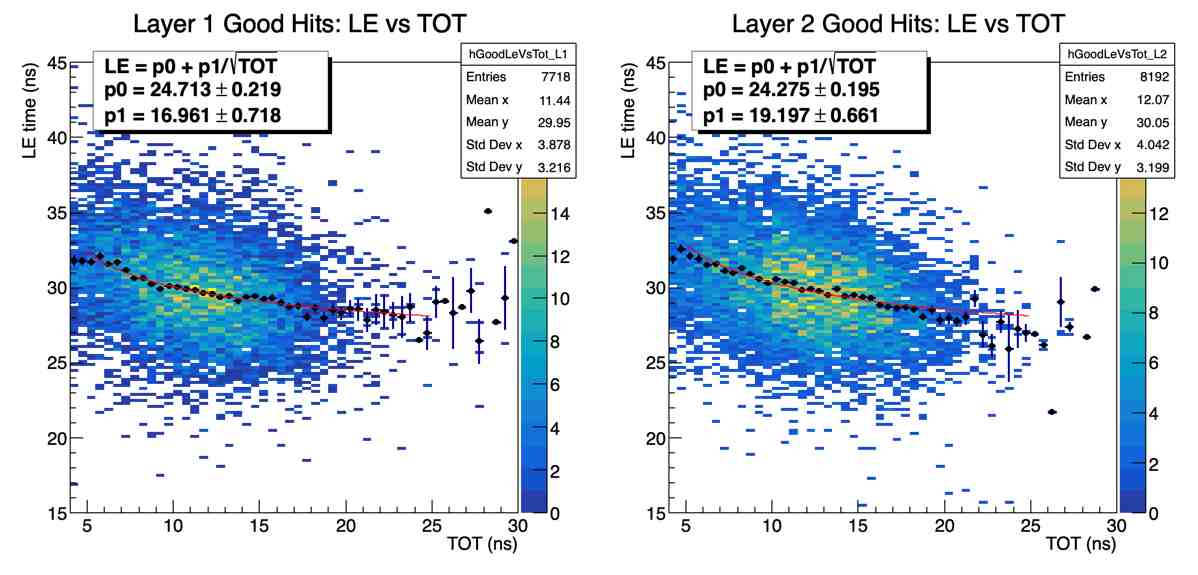
\includegraphics[width=\linewidth,height=0.64\textheight,keepaspectratio]{assets/CDet_timewalk_before.jpg}

  \centering\scriptsize Cross-target Run 3575: after channel-offset and ECal-time corrections, before time-walk correction
  \column{0.40\textwidth}
  \begin{itemize}
    \item Budget constraints precluded ADC instrumentation.
    \item The NINO pulse width provides time over threshold, a proxy for pulse amplitude.
    \item Larger pulses (larger ToT) cross threshold earlier. Here, earlier arrival means a smaller LE time, hence the downward slope.
    \item ToT supports a useful time-walk correction, but it does not replace a calibrated charge measurement.
  \end{itemize}
  \vspace{0.2cm}
  \lesson{The calibration must recover stable timing from leading edge and ToT alone.}
\end{columns}
\end{frame}

% Suggested pace: 1:15
\begin{frame}{Calibration strategy}
\small
\begin{columns}[T,onlytextwidth]
  \column{0.47\textwidth}
  \textbf{Align the detector}
  \begin{itemize}
    \item Extract channel-level timing offsets with half-bar information as a robust fallback.
    \item Correct common ECal-time dependence with a fixed-effects treatment across half-bars.
    \item Apply a layer-dependent ToT correction.
  \end{itemize}
  \column{0.49\textwidth}
  \textbf{Build track candidates}
  \begin{itemize}
    \item Form pulses from matched leading and trailing edges.
    \item Pair hits across the two CDet layers using timing and an ECal-projected trajectory.
    \item Retain exclusive single-layer candidates when one layer has no compatible hit.
  \end{itemize}
\end{columns}
\vspace{0.25cm}
\begin{block}{Corrected timing observable}
\centering
$t_{\mathrm{corr}}=t_{\mathrm{LE}}+\Delta t_{\mathrm{channel}}+\Delta t_{\mathrm{ECal}}+\Delta t_{\mathrm{ToT}}+\Delta t_{\mathrm{run}}$
\end{block}
\end{frame}

% Suggested pace: 1:05
\begin{frame}{Corrected timing and trajectory identify high-energy electrons}
\begin{columns}[T,onlytextwidth]
  \column{0.58\textwidth}
  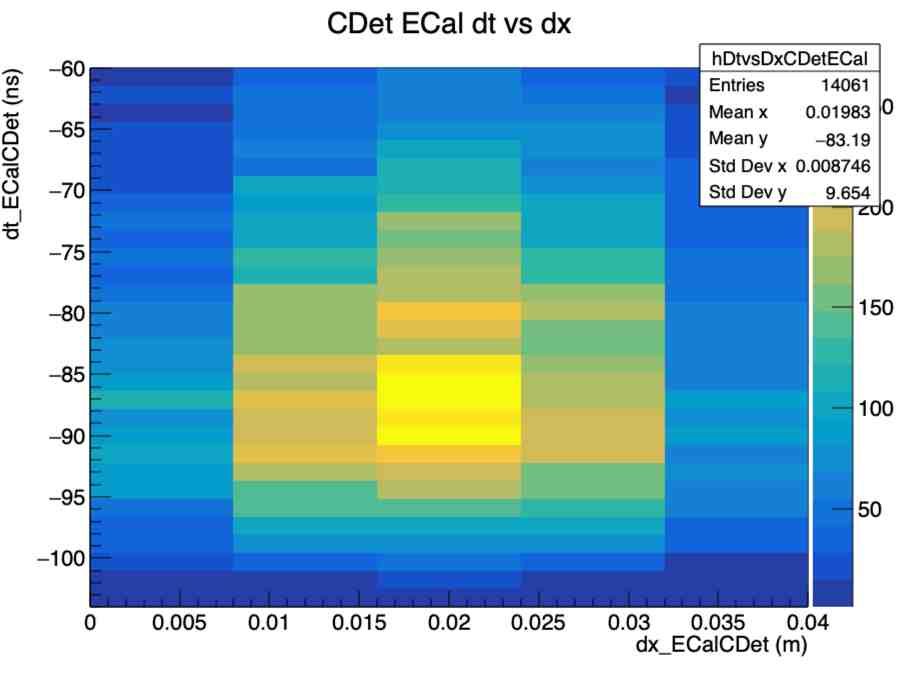
\includegraphics[width=\linewidth,height=0.66\textheight,keepaspectratio]{assets/CDet_Run6077_dt_vs_dx.jpg}

  \centering\scriptsize Run 6077, LH$_2$; accepted two-layer pairs combined across CDet
  \column{0.38\textwidth}
  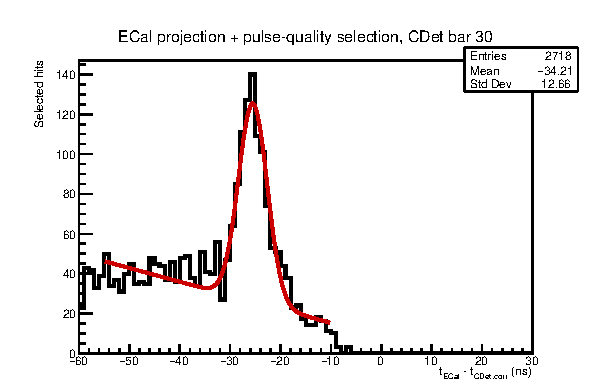
\includegraphics[width=\linewidth,height=0.35\textheight,keepaspectratio]{assets/CDet_Run6077_Bar030_TimingPeak.pdf}

  \centering\scriptsize Bar 30: ECal projection and pulse-quality selection

  \raggedright\normalsize
  \begin{itemize}
    \item High-energy electron candidates use ECal/HCal coincidence timing; the ECal position predicts the trajectory through CDet.
    \item Good CDet pairs form a compact locus in corrected time and $\Delta x$, rejecting the broad accidental background.
  \end{itemize}
\end{columns}
\end{frame}

% Suggested pace: 1:00
\begin{frame}{Current CDet timing and transverse-position resolution}
\small
\begin{columns}[T,onlytextwidth]
  \column{0.48\textwidth}
  \centering
  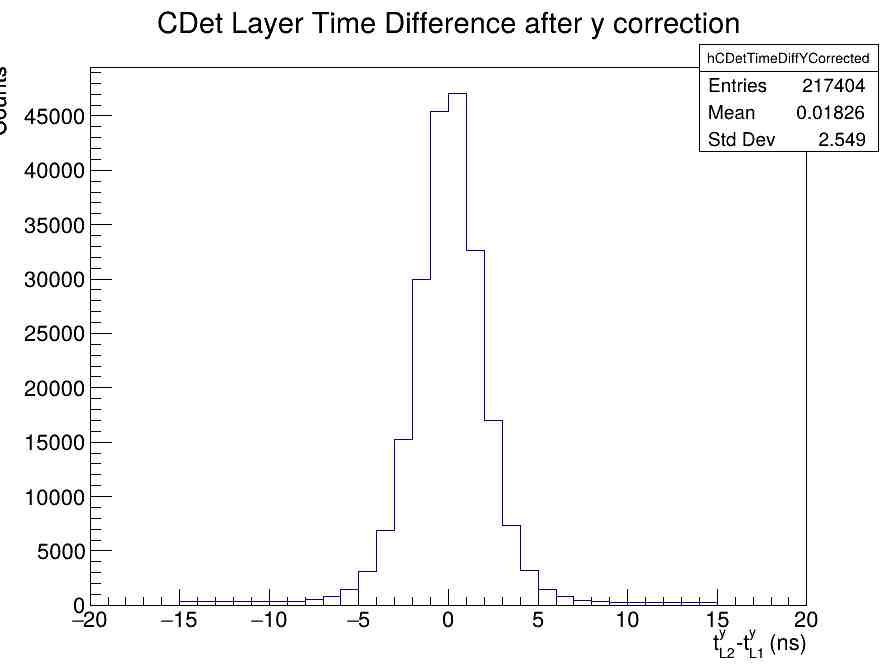
\includegraphics[width=\linewidth,height=0.43\textheight,keepaspectratio]{assets/CDet_Run5710_LayerTimeDifference.jpg}

  \textbf{$\sigma(t_{L2}-t_{L1})=2.55$ ns RMS}

  \vspace{0.08cm}
  \scriptsize Run 5710 cross-target; corrected accepted pairs

  \vspace{0.14cm}
  \normalsize
  Equal, independent layers would give
  $\sigma_t\approx 2.55/\sqrt{2}=1.80$ ns per layer.

  \column{0.48\textwidth}
  \centering
  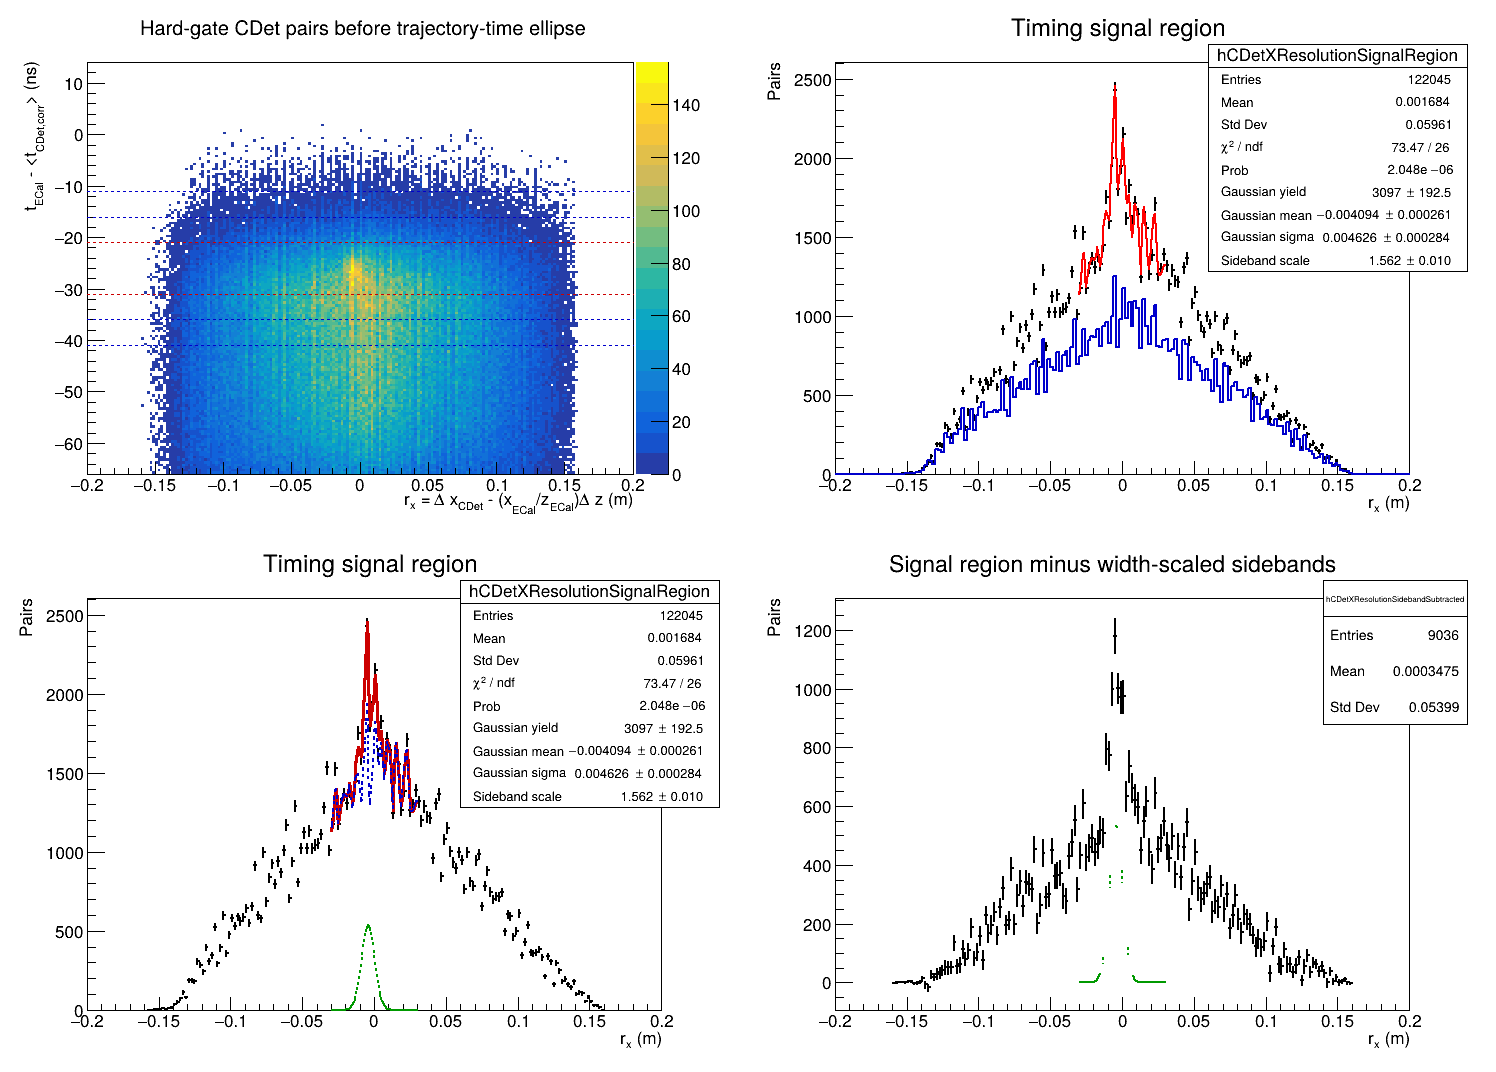
\includegraphics[width=\linewidth,height=0.43\textheight,keepaspectratio,trim=720 540 0 0,clip]{assets/CDet_Run6077_XResolutionStudy.png}

  \textbf{$\sigma(r_x)=4.63\pm0.28$ mm}

  \vspace{0.08cm}
  \scriptsize Run 6077 LH$_2$; timing-sideband constrained fit

  \vspace{0.14cm}
  \normalsize
  $r_x=(x_{L2}-x_{L1})-(x_{\rm ECal}/z_{\rm ECal})\Delta z$.
  Equal, independent layers imply a preliminary
  $\sigma_x\approx 3.3$ mm scale per layer.
\end{columns}
\end{frame}

% Suggested pace: 1:00
\begin{frame}{CDet information now reaches the front-tracker ROI}
\small
\begin{columns}[T,onlytextwidth]
  \column{0.66\textwidth}
  \begin{overpic}[width=\linewidth]{assets/Run5711_event38340.jpeg}
    \put(7,50){\colorbox{white}{\textbf{ECal}}}
    \put(18,50){\colorbox{white}{\textbf{CDet}}}
    \put(59,44){\colorbox{white}{\textbf{GEMs}}}
    \put(82,60){\colorbox{white}{\textbf{HCal}}}
  \end{overpic}

  \centering\scriptsize Run 5711 event 38340, one of the 117 CDet--GEM overlap events
  \column{0.30\textwidth}
  \footnotesize
  \begin{itemize}
    \item ECal and CDet define electron-ray hypotheses across the target.
    \item The replay exports ordinary pairs, seam pairs, and exclusive single-layer hypotheses.
    \item In a 261,010-event Run 5711 sample, 117 events contain both a front-GEM track and a CDet hypothesis.
  \end{itemize}
  \vspace{0.12cm}
  \begin{block}{Current status}
    The hypotheses support validation and diagnostics. They do not yet constrain production GEM pattern recognition.
  \end{block}
\end{columns}
\end{frame}

% Suggested pace: 1:00, leaving about 0:20 margin
\begin{frame}{Status and next steps}
\begin{columns}[T,onlytextwidth]
  \column{0.50\textwidth}
  \textbf{Completed}
  \begin{itemize}
    \item Timing calibration from TDC leading edge and ToT
    \item Detector-local pair and single-layer reconstruction
    \item ECal-projected trajectory matching
    \item CDet hypothesis export to FTROI
  \end{itemize}
  \column{0.46\textwidth}
  \textbf{In progress}
  \begin{itemize}
    \item Complete the target-coordinate transformation
    \item Validate elastic closure against reconstructed front-GEM tracks
    \item Quantify background rejection and GEM ROI reduction
    \item Measure any reconstruction-time improvement
  \end{itemize}
\end{columns}
\vspace{0.3cm}
\begin{block}{Takeaway}
\centering
CDet turns a very high-occupancy timing detector into usable electron-track constraints for GEp-V elastic-event reconstruction.
\end{block}
\end{frame}

\end{document}
